\documentclass[11pt]{article} 
\usepackage[english]{babel}
\usepackage[utf8]{inputenc}
\usepackage[margin=0.5in,top=0.5in,bottom=0.75in]{geometry}
\usepackage{amsmath}
\usepackage{amsthm}
\usepackage{amsfonts}
\usepackage{amssymb}
\usepackage[usenames,dvipsnames]{xcolor}
\usepackage{graphicx}
\usepackage[siunitx]{circuitikz}
\usepackage{tikz}
\usepackage[colorinlistoftodos, color=orange!50]{todonotes}
\usepackage{hyperref}
\usepackage[numbers, square]{natbib}
\usepackage{fancybox}
\usepackage{epsfig}
\usepackage{soul}
\usepackage[framemethod=tikz]{mdframed}
\usetikzlibrary{positioning, automata, backgrounds}
\usepackage{tikz}\usetikzlibrary{arrows.meta,backgrounds,calc,quotes}
\usepackage[shortlabels]{enumitem}
\usepackage[version=4]{mhchem}
\usepackage{multicol}
\usepackage{forest}
\usepackage{mathtools}
\usepackage{comment}
\usepackage{enumitem}
\usepackage[utf8]{inputenc}
\usepackage[linesnumbered,ruled,vlined]{algorithm2e}
\usepackage{listings}
\usepackage{color}
\usepackage[numbers]{natbib}
\usepackage{subfiles}
\usepackage{tkz-berge}
\usepackage{mathtools}
\DeclarePairedDelimiter\ceil{\lceil}{\rceil}
\DeclarePairedDelimiter\floor{\lfloor}{\rfloor}



\newtheorem{prop}{Proposition}[section]
\newtheorem{thm}{Theorem}[section]
\newtheorem{lemma}{Lemma}[section]
\newtheorem{cor}{Corollary}[prop]

\theoremstyle{definition}
\newtheorem{definition}{Definition}

\theoremstyle{definition}
\newtheorem{required}{Problem}
\newtheorem*{requiredHC}{Problem HC}


\theoremstyle{definition}
\newtheorem{ex}{Example}

\newcommand{\interval}[4]{\draw (#2, #1) -- (#3, #1); % Usage: \interval{height}{start}{end}{label}
\draw (#2, #1-0.11) -- (#2, #1+0.11); % draw left whisker
\draw (#3, #1-0.11) -- (#3, #1+0.11); % draw right whisker
\node[] at (#2-0.25, #1) {#4};
}

\tikzset{>={Stealth[length=7pt]}}
\tikzset{
    vertex/.style={circle,draw,minimum size=16,inner sep=0pt,font=\normalsize},
    edgelabel/.style={rectangle,draw=none,font=\footnotesize,outer sep=0pt},
    every node/.style={vertex},
    every edge quotes/.append style={edgelabel},
    every to/.append style={every node/.style={edgelabel}},
    wide/.style={line width=4pt,>={Stealth[length=18pt]}},
    directed/.style={arrows={->},font=\small},
    caption/.style={text width=6cm,align=center,rectangle,draw},
}


\setlength{\marginparwidth}{3.4cm}
%#########################################################

%To use symbols for footnotes
\renewcommand*{\thefootnote}{\fnsymbol{footnote}}
%To change footnotes back to numbers uncomment the following line
%\renewcommand*{\thefootnote}{\arabic{footnote}}

% Enable this command to adjust line spacing for inline math equations.
% \everymath{\displaystyle}

% _______ _____ _______ _      ______ 
%|__   __|_   _|__   __| |    |  ____|
%   | |    | |    | |  | |    | |__   
%   | |    | |    | |  | |    |  __|  
%   | |   _| |_   | |  | |____| |____ 
%   |_|  |_____|  |_|  |______|______|
%%%%%%%%%%%%%%%%%%%%%%%%%%%%%%%%%%%%%%%

\title{
\normalfont \normalsize 
\textsc{CSCI 3104 Fall 2022 \\ 
Instructors: Prof. Grochow and Chandra Kanth Nagesh} \\
[10pt] 
\rule{\linewidth}{0.5pt} \\[6pt] 
\huge Problem Set 9 \\
\rule{\linewidth}{2pt}  \\[10pt]
}
%\author{}
\date{}

\begin{document}

\definecolor{processblue}{cmyk}{0.96,0,0,0}
\definecolor{processred}{rgb}{200, 0, 0}
\definecolor{processgreen}{rgb}{0, 255, 0}
\DeclareGraphicsExtensions{.png}
\DeclareGraphicsExtensions{.gif}
\DeclareGraphicsExtensions{.jpg}

\maketitle


%%%%%%%%%%%%%%%%%%%%%%%%%
%%%%%%%%%%%%%%%%%%%%%%%%%%
%%%%%%%%%%FILL IN YOUR NAME%%%%%%%
%%%%%%%%%%AND STUDENT ID%%%%%%%%
%%%%%%%%%%%%%%%%%%%%%%%%%%
\noindent
Due Date \dotfill November 7, 2022 \\
Name \dotfill \textbf{Tyler Huynh} \\
Student ID \dotfill \textbf{109603994} \\
Collaborators \dotfill \textbf{N/A}

\tableofcontents

\section*{Instructions}
\addcontentsline{toc}{section}{Instructions}
 \begin{itemize}
	\item The solutions \textbf{must be typed}, using proper mathematical notation. We cannot accept hand-written solutions. Useful links and references on \LaTeX can be found \href{https://canvas.colorado.edu/courses/75824/pages/latex}{here on Canvas}.
	\item You should submit your work through the \textbf{class Canvas page} only. Please submit one PDF file, compiled using this \LaTeX \ template.
	\item You may not need a full page for your solutions; pagebreaks are there to help Gradescope automatically find where each problem is. Even if you do not attempt every problem, please submit this document with no fewer pages than the blank template (or Gradescope has issues with it).

	\item You are welcome and encouraged to collaborate with your classmates, as well as consult outside resources. You must \textbf{cite your sources in this document.} \textbf{Copying from any source is an Honor Code violation. Furthermore, all submissions must be in your own words and reflect your understanding of the material.} If there is any confusion about this policy, it is your responsibility to clarify before the due date. 

	\item Posting to \textbf{any} service including, but not limited to Chegg, Reddit, StackExchange, etc., for help on an assignment is a violation of the Honor Code.

	\item You \textbf{must} virtually sign the Honor Code (see Section \hyperlink{HonorCode}{Honor Code}). Failure to do so will result in your assignment not being graded.
\end{itemize}


\section*{Honor Code (Make Sure to Virtually Sign the Honor Pledge)} 
\addcontentsline{toc}{section}{Honor Code (Make Sure to Virtually Sign the Honor Pledge)}
\hypertarget{HonorCode}{}

\begin{requiredHC}
On my honor, my submission reflects the following:
\begin{itemize}
\item My submission is in my own words and reflects my understanding of the material.
\item Any collaborations and external sources have been clearly cited in this document.
\item I have not posted to external services including, but not limited to Chegg, Reddit, StackExchange, etc.
\item I have neither copied nor provided others solutions they can copy.
\end{itemize}

\noindent In the specified region below, clearly indicate that you have upheld the Honor Code. Then type your name. 
\end{requiredHC}

\begin{proof}[Honor Code]
I, \textbf{Tyler Huynh} on my honor pledge that my submission is a reflection of my own understanding of the material, any and all collaborations/sources have been properly cited, I have not posted any material to external sources, and I have not copied other solutions as my own.
\end{proof}

\newpage
\section{Standard 23: Dynamic Programming: Using Recurrences to Solve}
Consider the \textsc{Knapsack} problem from lecture. Fill in the dynamic programming table for the following input: $[(1, 3), (2, 3), (2, 2), (3, 3), (4, 5)], W=7$. Here, each pair $(v_i, w_i)$ denotes an item with value $v_i$ and weight $w_i$. What is the value of the optimal knapsack choice? (You \textbf{do not} need to fill in back-pointers.)

\begin{proof}[Answer] Referenced: \textbf{https://www.youtube.com/watch?v=8LusJS5-AGot=490s}\\
%% YOU MAY FIND THE FOLLOWING TABLE FORMATTED IN LATEX USEFUL, THOUGH YOU'LL NEED TO CREATE MORE ROWS BY COPYING THE LINE "0 & & & & & & & &  \\ \hline"
I will first specify what the items, weight, and values are for our input: \\
\begin{center}
Items: 1, 2 ,3, 4, 5 \\
Values: 1, 2, 2, 3, 4 \\
Weights: 3, 3, 2, 3, 5 \\
\end{center}
I will now fill in our table to find he most optimal knapsack code, as follows: \\
\begin{tabular}{|r|c|c|c|c|c|c|c|c|}
\hline
& 0& 1& 2& 3& 4& 5& 6& 7 \\ 
 \hline
0 & 0 & 0 & 0 & 0 & 0 & 0 & 0 & 0  \\ 
\hline
(2, 2) 1 & 0 & 0 & 2 & 2 & 2 & 2 & 2 & 2  \\ 
\hline
(1, 3) 2 & 0 & 0 & 2 & 2 & 2 & 3 & 3 & 3  \\ 
\hline
(2, 3) 3 & 0 & 0 & 2 & 2 & 2 & 4 & 4 & 4  \\ 
\hline
(3, 3) 4 & 0 & 0 & 2 & 3 & 3 & 5 & 5 & 5  \\ 
\hline
(4, 5) 5 & 0 & 0 & 2 & 3 & 3 & 5 & 5 & 6  \\ 
\hline
\end{tabular}\\


%%%%%%%%%%%%%%%%%%%%%%%%%%%%%%%%%%%%%%%%%%%%%%%%%%
% YOUR ANSWER GOES HERE                          %
%%%%%%%%%%%%%%%%%%%%%%%%%%%%%%%%%%%%%%%%%%%%%%%%%%
From the above we can see that the most optimal knapsack choice would be 6.
\end{proof}

\newpage
\section{Standard 24: Backtracking to find Solutions}
Consider the \textsc{Knapsack} problem, with input $[ (5, 3), (6, 4), (3, 3), (7, 5),(5, 3)], W=9$. Here, each pair $(v_i, w_i)$ denotes an item with value $v_i$ and weight $w_i$. The following is the dynamic programming table for the optimum value. From the table, \textbf{clearly indicate the steps you take to backtrace to find the optimum knapsack.} Be sure to include the steps at which an item was \emph{not} chosen, as well as those at which it was chosen. That is, the number of steps your algorithm takes should be the same as the length of the list (5) (or maybe 6, depending on how you handle the last step). 


\begin{tabular}{|r|c|c|c|c|c|c|c|c|c|c|}
\hline
           & 0 & 1 & 2 & 3 & 4 & 5 & 6 & 7 & 8 & 9\\ \hline
0         & 0 & 0 & 0 & 0 & 0 & 0 & 0 & 0 & 0 & 0 \\ \hline
(5,3) 1 & 0 & 0 & 0 & 5 & 5 & 5 & 5 & 5 & 5 & 5  \\ \hline
(6,4) 2 & 0 & 0 & 0 & 5 & 6 & 6 & 6 &11&11& 11\\ \hline
(3, 3) 3& 0 & 0 & 0 & 5 & 6 & 6 & 8 &11&11& 11 \\ \hline
(7, 5) 4& 0 & 0 & 0 & 5 & 6 & 7 & 8 &11 &12& 13\\ \hline
(5, 3) 5 &0 & 0 & 0 & 5 & 6 & 7 &10&11& 12& 13\\ \hline
\end{tabular}

\begin{proof}[Answer]
I have also included how I backed tracked to find the most optimum knapsack, the circles represent the items I \textbf{took} and the arrows represent the path that I took. \\
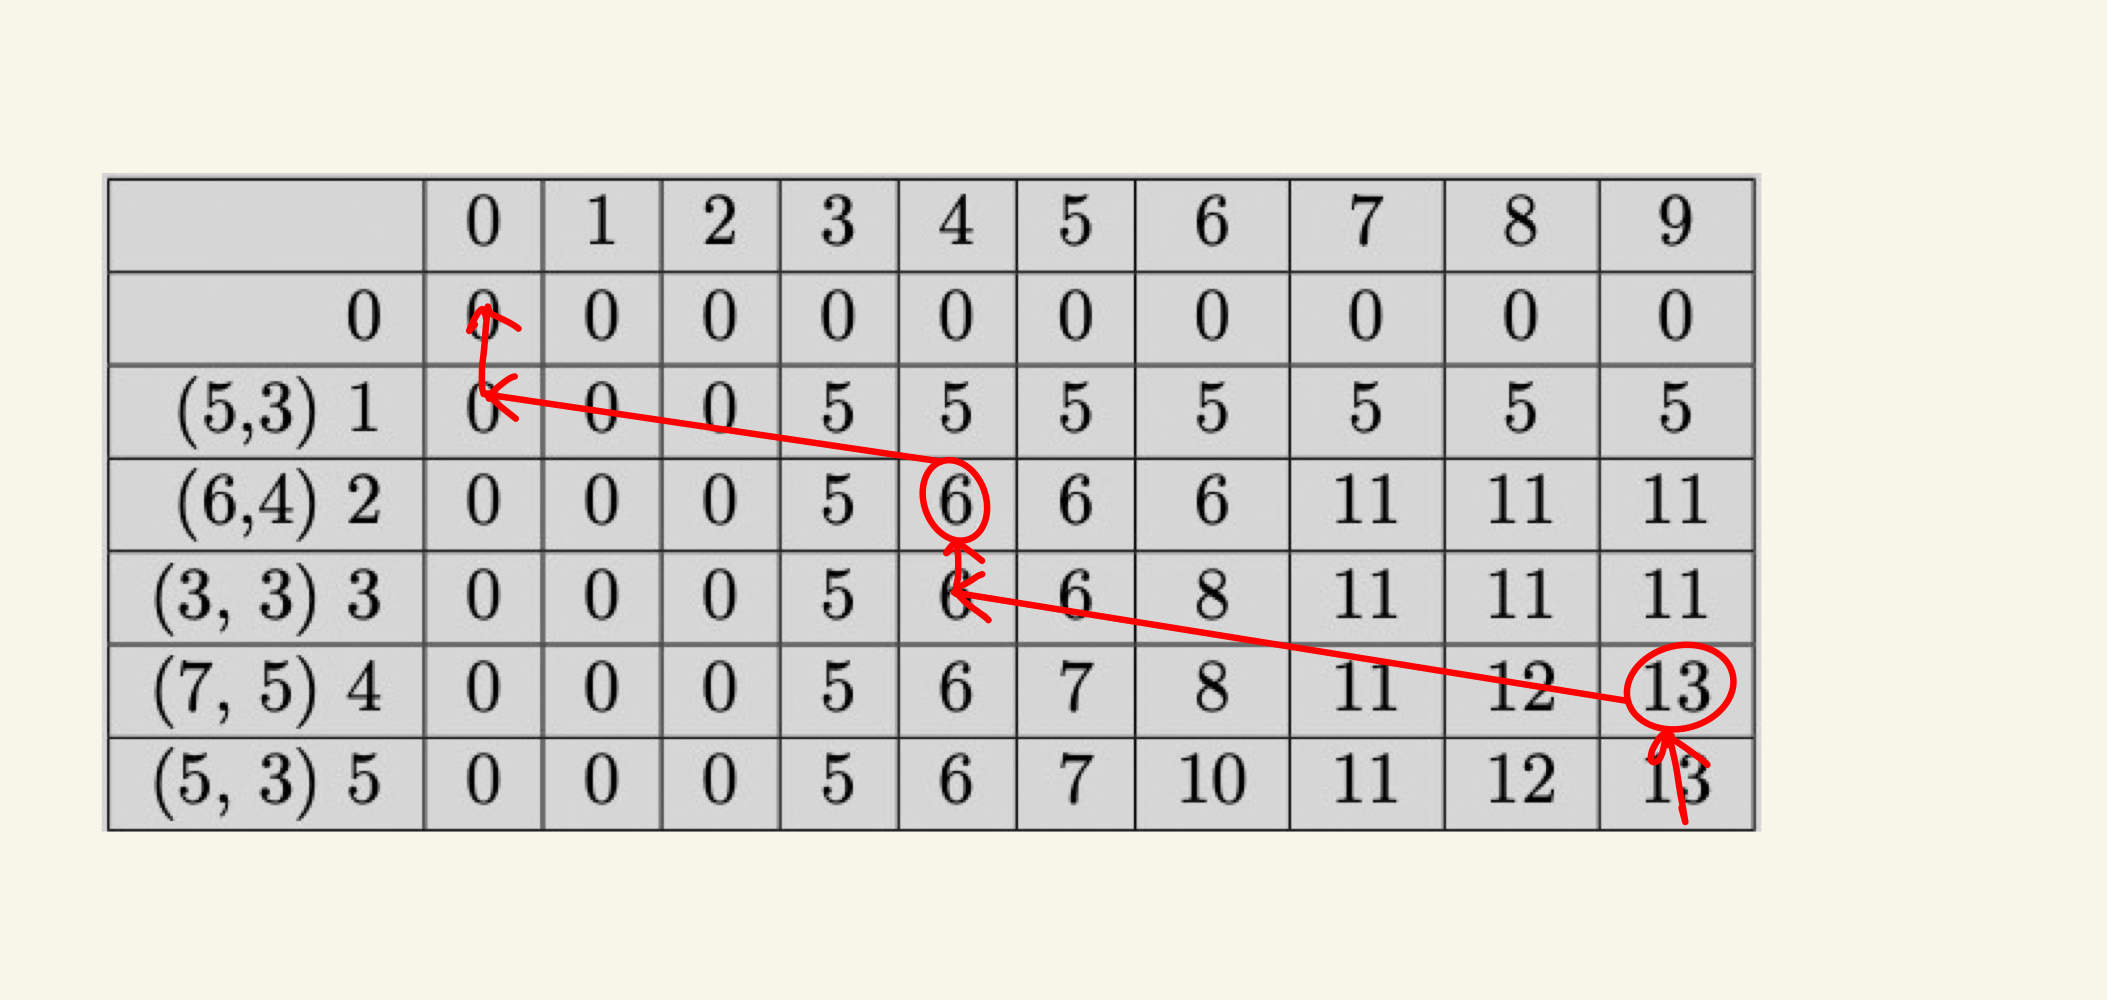
\includegraphics[width=0.6\textwidth]{IMG_5D67C562AAD8-1.jpeg}\\
The steps to backtrack to find the optimum knapsack will be: \\
\begin{itemize}
\item1. = \textrm{The first step we would take would be to compare item 5 at column 9 with the row above it, we can see that since these two values are equal to each other we would \textbf{not} take it.} \\
\item2. = \textrm{The second step we would take would be to compare item 4 at column 9 with the row above it, we can see that since these two values are \textbf{ not equal} to each other than we will traverse 5 towards the left side of our table.} \\
\item3. = \textrm{The third step we would take would be to compare item 3 at column 4 with the row above it, we can see that since these two values are equal to each other we would \textbf{not} take it.} \\
\item4. = \textrm{The fourth step we would take would be to compare item 2 at column 4 with the row above it, we can see that since these two values are \textbf{ not equal} to each other than we will traverse 4 towards the left side of our table.} \\
\item5. = \textrm{The fifth step we would take would be to compare item 1 at column 0 with the row above it, we can see that since these two values are equal to each other we would \textbf{not} take it.} \\
\textrm{From the above we have finished backtracking.}
\end{itemize}
We can see that the most optimum knapsack would be: \\
13 where we take item 4 with value and weight (7, 5) and item 2 with value and weight (6, 4).
\end{proof}

\newpage
\section{Standard 25: Design a Dynamic Programming Algorithm (Synthesis Standard)}

\begin{required}
Recall from class that if $x$ is a string, then a \emph{subseequence} of $x$ is a string of characters that occur in the same order as they do in $x$, but not necessarily contiguously. For example, $abc$ is a subsequence of $aebeec$, but $bca$ is not.

The \textsf{Longest Reflective Subsequence} problem is defined as follows.
\begin{itemize}
\item \textsf{Input:} A string $x$ with characters from a finite alphabet $\Sigma$
\item \textsf{Output:} A subsequence $y$ of $x$ such that for all $i \in \{1, \ldots, \ell=len(y)\}$, $y_{i} = y_{\ell - i + 1}$, that is as long as possible.
\end{itemize}

\textbf{Examples.} 
\begin{enumerate}
\item Any subsequence of length 0 (the empty string) or length 1 (a single character) is reflective.

\item In $abasd;klfjasd;lfkjba$, the first two and last two characters together form a reflective subsequence $abba$. There are also several reflective subsequences of length 6, for example, $abjjba$, $abffba$, $abddba$, $ab;;ba$, $abkkba$. The longest are of length 9, for example $abkfdfkba$.

\item In 12\textbf{3}4\textbf{5}67\textbf{89853}5, the longest reflective subsequence is $3589853$, which we've put in \textbf{bold} in the original string.
\end{enumerate}


\noindent \\ The goal of this problem is to design a dynamic programming algorithm to solve the \textsf{Longest Reflective Subsequence} problem.

\begin{enumerate}[label=(\alph*)]
\subsection{Problem 25\ref{2a}}
\item \label{2a} Let $L[i, j]$ denote the length of the longest reflective subsequence of $x[i, \ldots, j]$. Write down a mathematical recurrence for $L[i, j]$. Clearly justify each case.

\begin{proof}[Answer] Referenced \textbf{https://www.geeksforgeeks.org/longest-palindromic-subsequence-dp-12/} \\

For this problem we can see that the subproblem will be to denote the length of the longest reflective subsequence of $x[i, \ldots, j]$.
From this I will write down a recurrence for $L[i, j]$, such that: \\
Let n equal the length of the string.
\begin{align*}
L[i, j] = \begin{cases}
0 &: n = 0 \\
1 &: i = j \\
2 &: x_i = x_j, j-i \leq 1\\
L[i + 1, j - 1] + 2 &: x_i = x_j, j-1 > 1\\
max[L(i + 1, j), (i, j - 1)] &:  x_i \neq x_j
\end{cases}
\end{align*}
I will now explain how I came to each of the cases above: \\
\begin{itemize}
\item \textbf{Base Cases:} \\
For this case by the definition of the problem at hand we can see that if the length of the subsequence were to be of length 0 or of length 1 than the entirety of the subsequence is reflective. If it is of length 0 than we have a reflective subsequence of an empty string, if it is equal to 1 than we have a reflective subsequence of just that 1 character.\\

Another base case would be when the entries in the subsequence are the same, but the index of the characters are right next to each other such that it results in it being 2. \\
\item \textbf{Case 1} \\
For case 1 we can see that for this case they are the same character meaning that $x_i=x_j$, but there is at least one character that exists in between these indexes, such that: \\
\begin{center}
$L[i + 1, j - 1] + 2$
\end{center}
From the above we can see that if we increment $i$ by 1 and subtract $j$ by 1 we are looking at the string that does not include $x_i$ or $x_j$ since we know that the subsequence will already have these characters within it hence us adding two to it. \\
\item \textbf{Case 2:} \\
For case 2 we can see that for this case we are trying to find the max of the longest reflective subsequence when the characters $x_i$ and $x_j$ are not equal so they both cannot be included in the subsequence , such that: 
\begin{center}
$max(L[i + 1, j], L[i, j - 1]) $
\end{center}
From the above we can see that if since we are trying to find the max of the longest reflective subsequence, where we are looking at the longest reflective subsequence in the substring where we do not include $i$ and the longest subsequence in the substring where we do not include $j$ since .
\end{itemize}
\end{proof}



\newpage
\subsection{Problem 25\ref{2b}}
\item \label{2b} Clearly describe how to construct and fill in the lookup table. For the cell $L[i, j]$, clearly describe the sub-cases we consider (e.g., using a dependency diagram), which optimal sub-case we select, and any relevant pointers that should be included in the table of back-pointers.

\begin{proof}[Answer]
For the cell of $L[i, j]$, the sub-cases that we have to consider is that if the the subsequence is of length 0 than we have a reflective subsequence of an empty string, if it is of length 1 than we have a reflective subsequence of just 1 character. \\

When the subsequence is of length 2 and when $x_i = x_j$ that is when the characters of $i$ and $j$ are the same and the indexes of the characters are next to each other. \\

When $x_i = x_j$, meaning they are the same character, another sub-case would be when we increment $i$ by 1 and subtract $j$ by 1 we are looking at the string that does not include $x_i$ or $x_j$ since we know that the subsequence will already have these characters within it hence we add two to the sub-sequence, since the characters are the same, which will be reflective. \\

The last sub-case that we have to consider is when $x_i \neq x_j$. We are looking at the longest reflective subseqeunce in the substring where we do not include $i$ and the longest subsequence in the substring where we do not include $j$, where we would be finding the max between the two. \\

For the lookup table, we will have the rows of the table as $i$ where $i$ is 0 to $n-1$ and the columns will be $j$ is 0 to $n-1$. $i$ indicates the starting index and $j$ indicates the ending index. The way that the lookup table will be filled is looking at the previous cases stated above to see what case will fit the most and calculate it. \\

The back-pointers that we would use is when we consider where the value came from by considering the above cases.
\end{proof}



\newpage
\subsection{Problem 25\ref{2c}}
\item \label{2c} Work through an example of your algorithm using the input string $x = \texttt{uzwfzbu} $. Clearly show how to recover an optimal solution by backtracing. You may hand-draw your table(s), but your explanation must be typed.

\begin{proof}[Answer]
I will now run the algorithm on the example input string $x = \texttt{uzwfzbu} $: \\

\begin{tabular}{|r|c|c|c|c|c|c|c|c|}
\hline
L[i, j]& 0, u& 1, z& 2, w& 3, f& 4, z& 5, b& 6, u \\ 
 \hline
0, u & 1 & 1 & 1 & 1 & 3 & 3 & 5  \\ 
\hline
1, z& x& 1 & 1 & 1 & 3 & 3 & 3   \\ 
\hline
2, w & x & x & 1 & 1 & 1 & 1 & 1   \\ 
\hline
3, f& x & x & x & 1 & 1 & 1 & 1   \\ 
\hline
4, z& x & x & x & x & 1 & 1 & 1   \\ 
\hline
5, b& x & x & x & x & x & 1 & 1   \\ 
\hline
6, u& x & x & x & x & x & x & 1   \\ 
\hline
\end{tabular} \\

From the above we can see that the combination of uz(possible options include f, w)zu would be the most optimal solution via backtracking, such that: \\
\begin {itemize}
\item \textbf{Step 1:} We will begin at i = 0 and j = 6 where we can see that 5 will be the longest reflective subsequence of the string $x = \texttt{uzwfzbu} $. \\

\item \textbf{Step 2:} We will back track by comparing $i = 0$ and $j = 6$ to the cell below it and the cell to the left of it, we can see that this is \textbf{not} equal to either so we will refer to our algorithm and see that since we got the value from case 1 from our recurrence relation where case 1 dictates that since $x_i$ and $x_j$ are of the same character, but we know that at least one character exists between these indexes. So we increment $i$ and decrement $j$ by 1, from here we are looking at a string that does not include either $x_i$ or $x_j$, since we know that these subsequence will already have these characters within it, so we add 2. From here we know that since we had to use case 1 from our recurrence relation we backtrack to $i = 1$ and $j = 5$. This means that both u's is in the longest reflective subsequence so our current subsequence is uu.\\

\item \textbf{Step 3:} We compare the index  $i = 2$ and $j = 5$, to the cell below it and the cell to the left of it. Since it is equal to the cell to the left of it, this index's value came from the cell at $i=1$, $j=4$. Hence we will backtrack to this cell to find the most optimal solution. \\

\item \textbf{Step 4:} We will now compare the index at $i = 1$ and $j = 4$, to the cell below it and to the left we can see that this value is not equal to either. This is case 1 where since $x_i=x_j$ are the same character, but there exists at least one character in between them. We must increment $i$ and decrement $j$ by 1, from here we are looking at a string that does not include either $x_i$ or $x_j$, since we know that these subsequence will already have these characters within it, so we add 2. From here we know that since we had to use case 1 from our recurrence relation we backtrack to $i = 2$ and $j = 3$. We also know that both z's must be in our subsequence. So, our current subsequence is uzzu.\\

\item \textbf{Step 5:} From here we compare the index of $i = 2$ and $j = 3$ to the cell below it and the cell to the left of it , we can see that since these values are equal, there exists two possible solutions here as the index of $i = 2$ and $j = 3$, got its values from either of these indexes since they are equal. 

\item \textbf{Step 6:} Here we can see that since we have backtracked, thus far we have reached the most optimal solution for the input string of $x = \texttt{uzwfzbu} $, such that the most optimal solution would be of length = 5. From our backtracking we can see that we chose both u's and both z's to be in our longest subsequence. However, since there are other characters in our string that could exist in between the two z's to make it a length of 5. Thus our final longest reflective subsequence could be of the following: uzwzu, uzfzu.

\end{itemize}
\end{proof}
\end{enumerate}
\end{required}

%%%%%%%%%%%%%%%%%%%%%%%%%%%%%%%%%%%%%%%%%%%%%%%%%%

\end{document} % NOTHING AFTER THIS LINE IS PART OF THE DOCUMENT